\documentclass{article}
\usepackage{graphicx}
\begin{document}
\section{Float Placement}
This document uses four standard float placement hints. The surrounding text is
long enough to encourage LaTeX to move figures between top, here, bottom, and
float pages when needed.

\begin{figure}[t]
\centering

\includegraphics[width=80pt]{pixel.png}
\caption{Top-oriented figure}
\end{figure}

Teams often compare pages after a float-heavy edit because small differences in
placement can cascade into later page breaks. This paragraph exists to give the
first figure ordinary text to anchor against while keeping the source simple.

\begin{figure}[h]
\centering
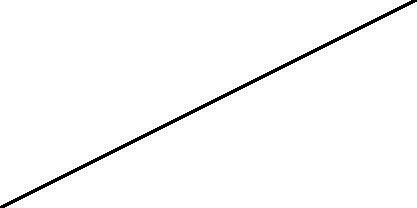
\includegraphics[width=140pt]{diagram.pdf}
\caption{Here-oriented figure}
\end{figure}

Additional filler text follows the second figure so the next float has room to
move. The benchmark does not need lorem ipsum; a short note about page flow is
enough to keep the output realistic.

\begin{figure}[b]
\centering

\includegraphics[width=90pt]{pixel.png}
\caption{Bottom-oriented figure}
\end{figure}

The remaining paragraph is intentionally longer. It describes how pagination can
change after a caption grows, a diagram is rescaled, or an inserted float forces
later material to slide onto the next page. All of those behaviors matter when a
parity harness compares a generated PDF with a reference rendering.

\begin{figure}[p]
\centering
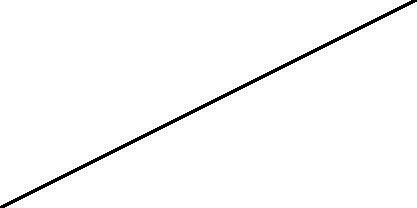
\includegraphics[width=0.7\textwidth]{diagram.pdf}
\caption{Dedicated float page candidate}
\end{figure}

\clearpage
This final sentence ensures the float page, if created, is followed by ordinary
body text in the compiled document.
\end{document}
